%%%%%%%%%%%%%%%%%%%%%%%%%%%%%%%%%%%%%%%%%%%%%%%%%%%%%%%%%%%%%%%%%
\subsubsection{Theorem 29}		%	TESTFÄLLE - RMed - Theorem 29
%%%%%%%%%%%%%%%%%%%%%%%%%%%%%%%%%%%%%%%%%%%%%%%%%%%%%%%%%%%%%%%%%

\noindent
Nach Theorem~\ref{theo: med_29} des Papers~\cite{meyer2} erreicht das Median Element für $k(n)=n / \log^{1/3}(n)$ und $d(n)=\log^{1/3}(n)$ eine erwartete \fg von $\mathbb{E}[f_{med}(n)]=\mO(\log\log(n))$ und alle übrigen Elemente eine erwartete \fg von $\mathbb{E}[f_{rem}(n)]=\mO(\sqrt{n})$.\\[.05cm]

\subsubsection*{\textit{Fragile complexity} des Median Elements}
Für die \fg des Medians \fgm lässt sich die Schranke aus Theorem~\ref{theo: med_29} trotz beschränkter Datenmenge eindeutig bestätigen.\\[.05cm]
In Abbildung~\ref{fig: med_theo29_med} zu sehen erkennt man schon bei direktem Vergleich zwischen den Experimentaldaten und der Funktion $f(x)=\log(x)$ der Daten die bestehende Korrelation. Parametrisiert man diese über einen Fit der Form $F(x)=a\cdot \log(x) + b$, so wie zu erkennen eine gute Übereinstimmung.

%---------------------------------------------------------------
%	FIG: FG COMP
\begin{figure}[H]
	\hspace*{-.9cm}
    \begin{minipage}[t]{.30\textwidth}
        \centering
		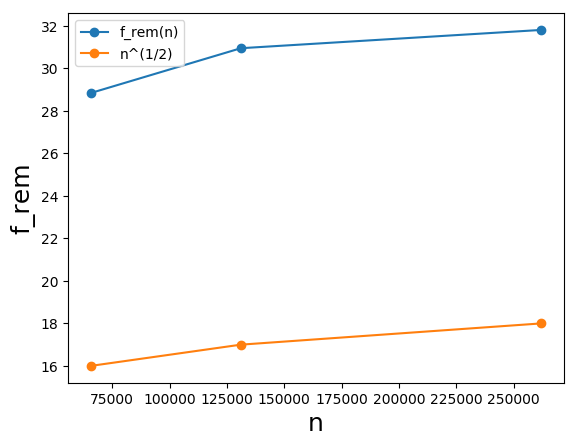
\includegraphics[width=0.95\textwidth]{pictures/med_algo_theo29_rem}
    \end{minipage}
    \hspace*{.3cm}
    \begin{minipage}[t]{.30\textwidth}
        \centering
        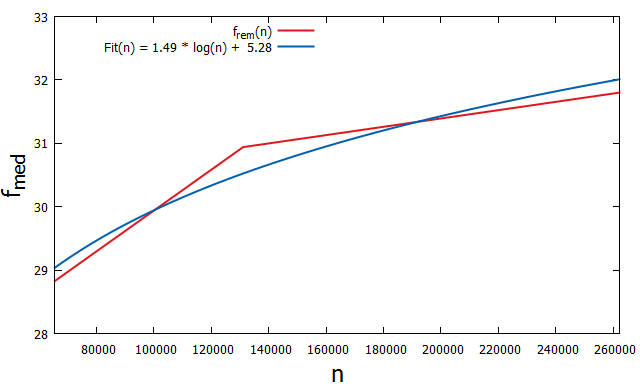
\includegraphics[width=1.25\textwidth]{pictures/med_algo_theo29_fit_rem}
    \end{minipage}
    \hspace*{1.2cm}
    \begin{minipage}[t]{.30\textwidth}
        \centering
        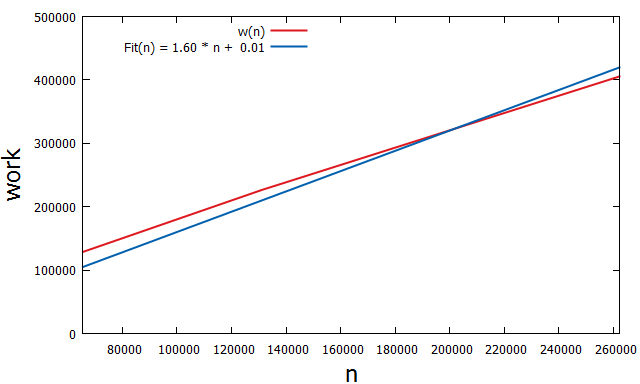
\includegraphics[width=1.25\textwidth]{pictures/med_algo_theo29_fit_work.png}
    \end{minipage}
    \vspace*{-0.1cm}
    \captionof{figure}{Vorhersage und Fit für \fgr sowie die Arbeit $w(n)$.}\label{fig: med_theo29_med}
\end{figure}

\noindent
Auch bei einer Parametrisierung nach Theorem~\ref{theo: med_29} wurde der Algorithmus \RM stets durch den \textit{AKS}-Algorithmus beendet. Um eine Abschätzung für die Wahrscheinlichkeit einer unglücklichen Wahl eines Samples der ersten Phase des Algorithmus zu liefern bedarf es einer deutlich umfangreicheren Datenmenge, so dass im Rahmen dieser Arbeit diesbezüglich keine Aussage getroffen werden kann. 


\subsubsection*{\textit{Fragile complexity} aller nicht-Median Elemente}
Abschließend untersuchen wir noch die \fg aller nicht-Median Elemente \fgr sowie die von dem Algorithmus \RM verrichtete Arbeit $w(n)$.\\[.05cm]
Wie in Abbildung~\ref{fig: med_theo29_rem} zu sehen ist bereits eine direkte Ähnlichkeit zwischen den Experimentaldaten und der Funktion $f(x)=\log(x)$ erkennbar. Wie zu erwarten konnte ein passender Fit der Form $F(n)= a\cdot \log(n) +b$ mit Parametern $a=1.49$ und $b=5.28$ berechnet werden.
%---------------------------------------------------------------
%	FIG: FG COMP
\begin{figure}[H]
	\hspace*{-0.9cm}
    \begin{minipage}[t]{.30\textwidth}
        \centering
		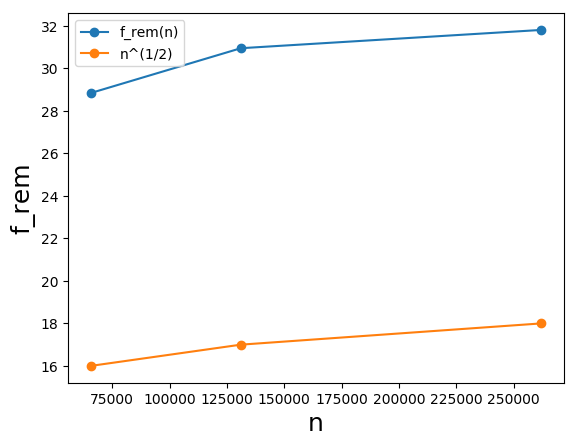
\includegraphics[width=0.95\textwidth]{pictures/med_algo_theo29_rem}
    \end{minipage}
    \hspace*{.3cm}
    \begin{minipage}[t]{.30\textwidth}
        \centering
        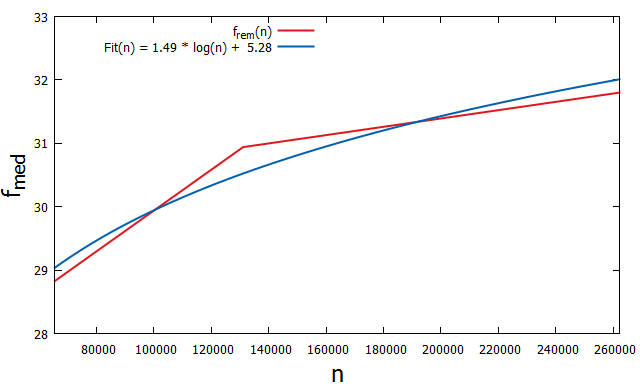
\includegraphics[width=1.25\textwidth]{pictures/med_algo_theo29_fit_rem}
    \end{minipage}
    \hspace*{1.2cm}
    \begin{minipage}[t]{.30\textwidth}
        \centering
        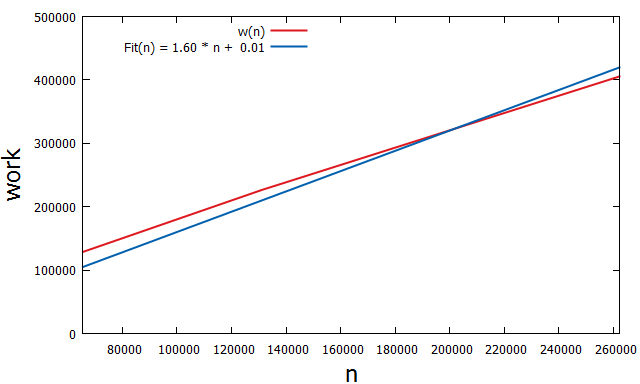
\includegraphics[width=1.25\textwidth]{pictures/med_algo_theo29_fit_work.png}
    \end{minipage}
    \vspace*{-0.1cm}
    \captionof{figure}{Vorhersage und Fit für \fgr sowie die Arbeit $w(n)$.}\label{fig: med_theo29_rem}
\end{figure}

\noindent
Zur Sicherheit wurde die verrichtete Arbeit $w(n)$ noch gegen einen Fit der Form $F(n)= a\cdot n + b$ abgeglichen, der einen nahezu deckungsgleiche Darstellung ergibt.


%---------------------------------------------------------------
\noindent